% \section{TAREAS}
% \begin{itemize}
%     % \item  \textbf{Hacer PPT para el personal del SENA}
%     \item  \textbf{Hacer resumen del trabajo para articulo cientifico}, formato genérico por el momento
%     % \item  \textbf{Hacer 
%     % formulario del trabajo (6 preguntas)}. Hablar  del modelado, del tabajo realizado y la precision del modelo. Posibilidad y trabajos futuros.
%     % \item Corregir preguntas formulario
%     % \item Cuadrar reunion (1 semana de anticipación)

% \end{itemize}

En este capítulo se presenta la evaluación del proyecto en cuanto al cumplimiento de los objetivos del proyecto, así como también con respecto a los análisis planteados en la etapa de preparación de datos y los resultados obtenidos. Para ello es importante citar nuevamente los objetivos específicos planteados al inicio del capítulo \ref{Objs}:

%\subsection{Objetivos Específicos 10 - 19}
\section{Objetivos específicos (OE)}\label{objesp}
\subsection{OE\#1: Identificar entradas, salidas, variables y parámetros asociados al sistema de producción ganadero objetivo.}

Teniendo en cuenta el proceso descriptivo realizado en los capítulos anteriores, se puede establecer que la información correspondiente al OE\#1 se encuentra resumido de la siguiente manera:

\subsubsection{Entradas}
Son las reses que participan en la producción de leche cruda. Así como también los insumos  que permiten el mantenimiento del CA-SENA-POP.

\subsubsection{Variables}
Las variables en cuestión son, por una parte, la cantidad de leche producida por una vaca durante un periodo de lactancia, por otra parte, la cantidad de peso de la reses productoras o no productoras; y por último, la cantidad de estiércol producido por el hato que será tratado para producir abono para el CA-SENA-POP.

\subsubsection{Salidas}

Las salidas del sistema productivo del CA-SENA-POP son la producción neta de leche cruda, la producción de carne de las reses vendidas y la producción de estiércol y materia fecal que es usado como abono en los distintos potreros internos en la finca del SENA en la ciudad de Popayán. La leche cruda es producida para posteriormente ser vendida para generar ganancias monetarias que serán reinvertidas en el CA-SENA-POP. La carne representa el peso final de la res parida, desteta, cebada o en proceso de venta. 

\subsubsection{Parámetros}

El sistema productivo del CA-SENA-POP depende del consumo nutricional del hato. Este consumo varía proporcionalmente al peso del animal y a su rendimiento productivo teniendo un rango de valores proporcionales que oscilan de la siguiente manera:
\begin{itemize}
    \item Forrajes y alimentos secos: Consumo que varía entre un 10 a 20 \% del peso del animal.
    \item Concentrado y suplementos: Consumo que varía entre un 1 a 5 \% del peso del animal.
    \item Agua: Consumo ``Ad libitum'', que varía entre un 5 a 12 \% del peso del animal
    \item Medicamentos: Varían según el estado de salud del animal. Se asume un estado de salud óptimo durante este trabajo de investigación.
\end{itemize}

\subsection{OE\#2: Identificar modelos dinámicos que permitan pronosticar la producción de un sistema ganadero objetivo.}

Tal y como se menciona en la sección \ref{dinamod}, soportado por \cite{shanks}, \cite{silvestre} y \cite{iran}, una forma de encontrar una representación de un sistema por EDOs, es mediante un balance de energía que involucre a las variables en cuestión. Por tal motivo, se puede considerar factible que el modelo de 2 dimensiones descrito en la sección \ref{edosec} satisface el pronóstico de la producción en el tiempo de las 3 variables presentes en el sistema.


\subsection{OE\#3: Implementar métodos de solución de los modelos dinámicos de producción ganadera seleccionados.}

Tal y como se concluye en la sección \ref{simulwp}, una vez que se considera que un modelo EDO puede representar el comportamiento de las variables del sistema, este modelo EDO puede ser resuelto mediante algoritmos numéricos avanzados tales como que pueden ser utilizados mediante librerías como ``Scipy'', en scripts de Python. Para este caso, el sistema modelado en cuestión representa un problema de valor inicial, por lo que puede ser resuelto mediante un método de solución como ``odeint'' o ``scipy.integrate''. El proceso en el que este algoritmo es usado para dar solución al modelo EDO a cada una de las producciones de las reses que pertenecen al sistema se encuentra descrito en la sección \ref{optimizodeint} o en mayor detalle en los scripts de python implementados en Jupyter-Anaconda \cite{msclfggrepo}.


\subsection{OE\#4: Evaluar la estimación de los modelos seleccionados comparando la solución con datos empíricos recogidos.} 

En cuanto a este objetivo, el modelo WP, planteado por el sistema de 2D de EDOs, descrito en el capítulo anterior tiene un desempeño deseado puesto que tal y como se describe en la sección \ref{}, los valores de los criterios BIC Y AIC son menores a medida que el modelo logra un ajuste más apropiado para cada una de las reses de cada parto. Adicionalmente, criterios como el $\chi^{2}$ reducido tienden a ser cada vez más próximo a 1 lo que complementa la afirmación anterior. Por último pero no menos importante, aún cuando esta última afirmación es netamente subjetiva, se puede observar que  cuando el modelo presenta características estadísticas como las previamente decsritas en este objetivo, el ajuste visual tiende a ser similar al comportamiento de los datos empíricos recogidos.



% \section{Objetivo General}
% Estructurar y evaluar un modelo dinámico que simule el comportamiento de sistemas de producción ganadera en el Centro Agropecuario del Servicio Nacional de Aprendizaje, ubicado en el municipio de Popayán, en departamento del Cauca (CA-SENA-POP).

\section{Metodología CRISP-DM}

En lo que respecta a la metodología de estudio, las actividades llevadas a cabo en las etapas de la metodología CRISP-DM descritas en los capítulos anteriores pueden ser justificantes suficientes para corroborar si se ha hecho un debido manejo y procesamiento de datos, en especial, porque cada una de las acciones realizadas al conjunto de datos base ha sido detallada y justificada en cada capítulo en pro de satisfacer los objetivos de este trabajo de grado.\\

En cuanto al primero objetivo, las etapas 1, 2 y 3 de la metodología CRISP-DM permiten identificar el contexto del CA-SENA-POP, así como también los recursos que participan en el proceso productivo del hato.\\

Para satisfacer el OE\#2, basta con realizar un proceso repetitivo entre las etapas 1, 2, 3 y 4; en pro de determinar los parámetros y variables que deben ser tenidos en cuenta al momento de realizar el ajuste de los datos a modelos EDO.\\

Por último pero no menos importante, el OE \#3 puede ser satisfecho una vez cumplidas las primeras 3 etapas de la metodología. Mientras que el OE \#4 podrá ser satisfecho en el transcurso de esta etapa de evaluación.


\subsection{CRISP-DM ETAPA\#4: Ajuste de curvas por métodos no lineales}

\begin{table}[H]
\centering
\caption{Comparación de error cuadrático medio MSE para cada método de ajuste no lineal.}
\label{msecompare}
\resizebox{\textwidth}{!}{%
\begin{tabular}{|ccccccc|}
\hline
\multicolumn{7}{|c|}{MSE} \\ \hline
\multicolumn{1}{|c|}{\multirow{2}{*}{MÉTODO}} &
  \multicolumn{6}{c|}{PARTO ($P\#_{i}$)} \\ \cline{2-7} 
\multicolumn{1}{|c|}{} &
  \multicolumn{1}{c|}{$P\#_{1}$} &
  \multicolumn{1}{c|}{$P\#_{2}$} &
  \multicolumn{1}{c|}{$P\#_{3}$} &
  \multicolumn{1}{c|}{$P\#_{4}$} &
  \multicolumn{1}{c|}{$P\#_{5}$} &
  $P\#_{6}$ \\ \hline
\multicolumn{1}{|c|}{\begin{tabular}[c]{@{}c@{}}LEVENBERG - MARQUARDT\\ FIT ÚNICO\end{tabular}} &
  \multicolumn{1}{c|}{6.8240} &
  \multicolumn{1}{c|}{17.8285} &
  \multicolumn{1}{c|}{21.4705} &
  \multicolumn{1}{c|}{12.4351} &
  \multicolumn{1}{c|}{11.3886} &
  4.8692 \\ \hline
\multicolumn{1}{|c|}{FIT MULTIPLE} &
  \multicolumn{1}{c|}{4.4826} &
  \multicolumn{1}{c|}{8.444} &
  \multicolumn{1}{c|}{12.7492} &
  \multicolumn{1}{c|}{8.7615} &
  \multicolumn{1}{c|}{9.4352} &
  4.7066 \\ \hline
\multicolumn{1}{|c|}{EFECTOS MIXTOS} &
  \multicolumn{1}{c|}{4.4855} &
  \multicolumn{1}{c|}{8.4482} &
  \multicolumn{1}{c|}{12.7476} &
  \multicolumn{1}{c|}{8.7735} &
  \multicolumn{1}{c|}{9.4402} &
  4.6487 \\ \hline
\end{tabular}%
}
\end{table}
\pagebreak

Para realizar una evaluación crítica respecto a los ajustes no lineales de las curvas de lactancia para determinar sí estos son representativos y significativos; es necesarios tener en consideración los criterios de MSE, RMSE, AIC, BIC de cada uno de los ajustes no lineales realizados. \\

En primera instancia, los ajustes no lineales realizados al inicio del capitulo \ref{crisp4} evidencian características estadísticas con valores relativamente bajos de MSE y RMSE (ver tabla \ref{msecompare}), así como también una reducción progresiva de los criterios AIC y BIC a medida que se comparan los métodos de ajuste de curvas por el algortimo de Levenberg-Marquardt o por efectos mixtos fijos y aleatorios no lineales  .\\

Por lo tanto, es plausible afirmar que los ajustes realizados presentan una buena bondad de ajuste. (Para mayor información respecto a los características estadísticas de cada ajuste, consultar en \cite{msclfggrepo}, el algoritmo ``AnaMixEffGenBeta2.m'' y comparar las variables STATSMEFIN, STATSNLME2, STATSNLME2RF y STATSNLME2RFPAT). \\

Adicionalmente, si no tenemos en cuenta la poca cantidad de valores atípicos existentes en los datos y evidenciados en los diagramas de cajas y bigotes (ver figura \ref{nlinfitbox1png}); se puede establecer que la gráfica de probabilidad normal de los residuos evidencian un acuerdo razonable con los supuestos del modelo sobre los errores (ver figura \ref{residprobnormpng}).\\

\textbf{OBS: } Tener en cuenta que estos de distribución de población y distribución de datos en diagrama de caja y bigotes son realizados para cada parto, pero no se incluyen en la monografía por temas de espacio)

\subsection{Producción neta real Vs Producción teórica por ajustes no lineales}

Podría considerarse que otra forma de establecer si los ajustes no lineales de los parámetros del modelo de Wood son acertados, es verificando el área bajo la curva que se genera por estos parámetros, es decir, la producción neta de la curva de lactancia formada por los parámetros ajustados al modelo matemático de Wood. Así pues, si se realiza una tabla en la que se consignen los valores de los parámetros ajustados para cada metodo no lineal, y se comparar con los valores reales de las producciones netas de cada vaca en cada parto, se puede establecer si los ajustes pueden o no representar los datos de cada vaca, y finalmente, representar al producción total del hato. Esta comparación puede apreciarse en la figura \ref{prodparamscomparepng}.\\

En esta misma figura se puede observar como el método no lineal que presenta mejor ajuste es el método de LM, el cual aunque no presenta los porcentaje de error más pequeños para todos los grupos de partos, si presenta un valor total más aproximado a la producción total de leche real basada en registros reales.



\pagebreak
\begin{figure}[H]
    \centering
    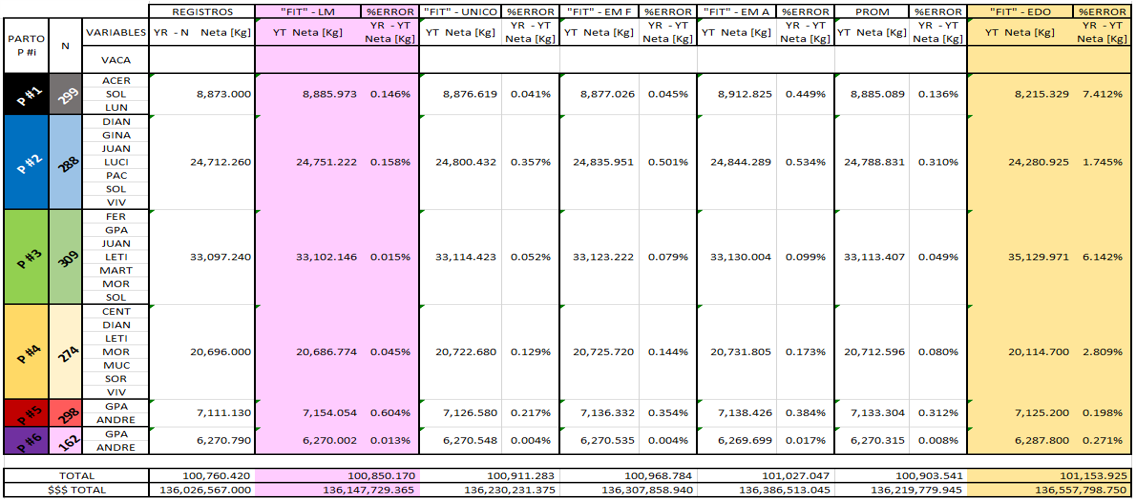
\includegraphics[angle=90, scale=0.69]{img/prodparamscompare.png}
    \caption{Comparación de producción real y teórica para cada método de ajuste no lineal. \label{prodparamscomparepng}}
\end{figure}
\pagebreak


% \begin{table}[]
% \centering
% \caption{Comparación de producción real y teoríca para cada méodo de ajuste no lineal}
% \label{prodparamscomparetab}
% \resizebox{\textwidth}{!}{%
% \begin{tabular}{lll|lllllllllllllll|}
% \cline{4-18}
%  &
%    &
%    &
%   \multicolumn{1}{l|}{REGISTROS} &
%   \multicolumn{1}{l|}{EMPÍRICOS} &
%   \multicolumn{1}{l|}{\%ERROR} &
%   \multicolumn{1}{l|}{"FIT" - LM} &
%   \multicolumn{1}{l|}{\%ERROR} &
%   \multicolumn{1}{l|}{"FIT" - UNICO} &
%   \multicolumn{1}{l|}{\%ERROR} &
%   \multicolumn{1}{l|}{"FIT" - EM F} &
%   \multicolumn{1}{l|}{\%ERROR} &
%   \multicolumn{1}{l|}{"FIT" - EM A} &
%   \multicolumn{1}{l|}{\%ERROR} &
%   \multicolumn{1}{l|}{PROM} &
%   \multicolumn{1}{l|}{\%ERROR} &
%   \multicolumn{1}{l|}{"FIT" - EDO} &
%   \%ERROR \\ \hline
% \multicolumn{1}{|l|}{\multirow{2}{*}{PARTO  $P \#_{i}$}} &
%   \multicolumn{1}{l|}{\multirow{2}{*}{N}} &
%   VARIABLES &
%   \multicolumn{1}{l|}{\begin{tabular}[c]{@{}l@{}}YR  - N\\ Neta {[}Kg{]}\end{tabular}} &
%   \multicolumn{1}{l|}{\begin{tabular}[c]{@{}l@{}}YT  \\ Neta {[}Kg{]}\end{tabular}} &
%   \multicolumn{1}{l|}{\begin{tabular}[c]{@{}l@{}}YR  - YT\\ Neta {[}Kg{]}\end{tabular}} &
%   \multicolumn{1}{l|}{\begin{tabular}[c]{@{}l@{}}YT  \\ Neta {[}Kg{]}\end{tabular}} &
%   \multicolumn{1}{l|}{\begin{tabular}[c]{@{}l@{}}YR  - YT\\ Neta {[}Kg{]}\end{tabular}} &
%   \multicolumn{1}{l|}{\begin{tabular}[c]{@{}l@{}}YT \\  Neta {[}Kg{]}\end{tabular}} &
%   \multicolumn{1}{l|}{\begin{tabular}[c]{@{}l@{}}YR  - YT\\ Neta {[}Kg{]}\end{tabular}} &
%   \multicolumn{1}{l|}{\begin{tabular}[c]{@{}l@{}}YT  \\ Neta {[}Kg{]}\end{tabular}} &
%   \multicolumn{1}{l|}{\begin{tabular}[c]{@{}l@{}}YR  - YT\\ Neta {[}Kg{]}\end{tabular}} &
%   \multicolumn{1}{l|}{\begin{tabular}[c]{@{}l@{}}YT \\  Neta {[}Kg{]}\end{tabular}} &
%   \multicolumn{1}{l|}{\begin{tabular}[c]{@{}l@{}}YR  - YT\\ Neta {[}Kg{]}\end{tabular}} &
%   \multicolumn{1}{l|}{\begin{tabular}[c]{@{}l@{}}YT \\  Neta {[}Kg{]}\end{tabular}} &
%   \multicolumn{1}{l|}{\begin{tabular}[c]{@{}l@{}}YR  - YT\\ Neta {[}Kg{]}\end{tabular}} &
%   \multicolumn{1}{l|}{\begin{tabular}[c]{@{}l@{}}YT \\  Neta {[}Kg{]}\end{tabular}} &
%   \begin{tabular}[c]{@{}l@{}}YR  - YT\\ Neta {[}Kg{]}\end{tabular} \\ \cline{3-18} 
% \multicolumn{1}{|l|}{} &
%   \multicolumn{1}{l|}{} &
%   VACA &
%   \multicolumn{15}{l|}{} \\ \hline
% \multicolumn{1}{|l|}{\multirow{3}{*}{$P\#_{1}$}} &
%   \multicolumn{1}{l|}{\multirow{3}{*}{299}} &
%   ACER &
%   \multicolumn{1}{l|}{\multirow{3}{*}{8873.000}} &
%   \multicolumn{1}{l|}{\multirow{3}{*}{7239.455}} &
%   \multicolumn{1}{l|}{\multirow{3}{*}{0.184}} &
%   \multicolumn{1}{l|}{\multirow{3}{*}{8885.973}} &
%   \multicolumn{1}{l|}{\multirow{3}{*}{0.146\%}} &
%   \multicolumn{1}{l|}{\multirow{3}{*}{8876.619}} &
%   \multicolumn{1}{l|}{\multirow{3}{*}{0.041\%}} &
%   \multicolumn{1}{l|}{\multirow{3}{*}{8877.026}} &
%   \multicolumn{1}{l|}{\multirow{3}{*}{0.045\%}} &
%   \multicolumn{1}{l|}{\multirow{3}{*}{8912.825}} &
%   \multicolumn{1}{l|}{\multirow{3}{*}{0.449\%}} &
%   \multicolumn{1}{l|}{\multirow{3}{*}{8885.089}} &
%   \multicolumn{1}{l|}{\multirow{3}{*}{0.136\%}} &
%   \multicolumn{1}{l|}{\multirow{3}{*}{8215.329}} &
%   \multirow{3}{*}{7.412\%} \\ \cline{3-3}
% \multicolumn{1}{|l|}{} &
%   \multicolumn{1}{l|}{} &
%   SOL &
%   \multicolumn{1}{l|}{} &
%   \multicolumn{1}{l|}{} &
%   \multicolumn{1}{l|}{} &
%   \multicolumn{1}{l|}{} &
%   \multicolumn{1}{l|}{} &
%   \multicolumn{1}{l|}{} &
%   \multicolumn{1}{l|}{} &
%   \multicolumn{1}{l|}{} &
%   \multicolumn{1}{l|}{} &
%   \multicolumn{1}{l|}{} &
%   \multicolumn{1}{l|}{} &
%   \multicolumn{1}{l|}{} &
%   \multicolumn{1}{l|}{} &
%   \multicolumn{1}{l|}{} &
%    \\ \cline{3-3}
% \multicolumn{1}{|l|}{} &
%   \multicolumn{1}{l|}{} &
%   LUN &
%   \multicolumn{1}{l|}{} &
%   \multicolumn{1}{l|}{} &
%   \multicolumn{1}{l|}{} &
%   \multicolumn{1}{l|}{} &
%   \multicolumn{1}{l|}{} &
%   \multicolumn{1}{l|}{} &
%   \multicolumn{1}{l|}{} &
%   \multicolumn{1}{l|}{} &
%   \multicolumn{1}{l|}{} &
%   \multicolumn{1}{l|}{} &
%   \multicolumn{1}{l|}{} &
%   \multicolumn{1}{l|}{} &
%   \multicolumn{1}{l|}{} &
%   \multicolumn{1}{l|}{} &
%    \\ \hline
% \multicolumn{1}{|l|}{\multirow{7}{*}{$P\#_{2}$}} &
%   \multicolumn{1}{l|}{288} &
%   DIAN &
%   \multicolumn{1}{l|}{\multirow{7}{*}{24712.260}} &
%   \multicolumn{1}{l|}{\multirow{7}{*}{22628.196}} &
%   \multicolumn{1}{l|}{\multirow{7}{*}{0.084}} &
%   \multicolumn{1}{l|}{\multirow{7}{*}{24751.222}} &
%   \multicolumn{1}{l|}{\multirow{7}{*}{0.158\%}} &
%   \multicolumn{1}{l|}{\multirow{7}{*}{24800.432}} &
%   \multicolumn{1}{l|}{\multirow{7}{*}{0.357\%}} &
%   \multicolumn{1}{l|}{\multirow{7}{*}{24835.951}} &
%   \multicolumn{1}{l|}{\multirow{7}{*}{0.501\%}} &
%   \multicolumn{1}{l|}{\multirow{7}{*}{24844.289}} &
%   \multicolumn{1}{l|}{\multirow{7}{*}{0.534\%}} &
%   \multicolumn{1}{l|}{\multirow{7}{*}{24788.831}} &
%   \multicolumn{1}{l|}{\multirow{7}{*}{0.310\%}} &
%   \multicolumn{1}{l|}{\multirow{7}{*}{24280.925}} &
%   \multirow{7}{*}{1.745\%} \\ \cline{2-3}
% \multicolumn{1}{|l|}{} &
%   \multicolumn{1}{l|}{} &
%   GINA &
%   \multicolumn{1}{l|}{} &
%   \multicolumn{1}{l|}{} &
%   \multicolumn{1}{l|}{} &
%   \multicolumn{1}{l|}{} &
%   \multicolumn{1}{l|}{} &
%   \multicolumn{1}{l|}{} &
%   \multicolumn{1}{l|}{} &
%   \multicolumn{1}{l|}{} &
%   \multicolumn{1}{l|}{} &
%   \multicolumn{1}{l|}{} &
%   \multicolumn{1}{l|}{} &
%   \multicolumn{1}{l|}{} &
%   \multicolumn{1}{l|}{} &
%   \multicolumn{1}{l|}{} &
%    \\ \cline{2-3}
% \multicolumn{1}{|l|}{} &
%   \multicolumn{1}{l|}{} &
%   JUAN &
%   \multicolumn{1}{l|}{} &
%   \multicolumn{1}{l|}{} &
%   \multicolumn{1}{l|}{} &
%   \multicolumn{1}{l|}{} &
%   \multicolumn{1}{l|}{} &
%   \multicolumn{1}{l|}{} &
%   \multicolumn{1}{l|}{} &
%   \multicolumn{1}{l|}{} &
%   \multicolumn{1}{l|}{} &
%   \multicolumn{1}{l|}{} &
%   \multicolumn{1}{l|}{} &
%   \multicolumn{1}{l|}{} &
%   \multicolumn{1}{l|}{} &
%   \multicolumn{1}{l|}{} &
%    \\ \cline{2-3}
% \multicolumn{1}{|l|}{} &
%   \multicolumn{1}{l|}{} &
%   LUCI &
%   \multicolumn{1}{l|}{} &
%   \multicolumn{1}{l|}{} &
%   \multicolumn{1}{l|}{} &
%   \multicolumn{1}{l|}{} &
%   \multicolumn{1}{l|}{} &
%   \multicolumn{1}{l|}{} &
%   \multicolumn{1}{l|}{} &
%   \multicolumn{1}{l|}{} &
%   \multicolumn{1}{l|}{} &
%   \multicolumn{1}{l|}{} &
%   \multicolumn{1}{l|}{} &
%   \multicolumn{1}{l|}{} &
%   \multicolumn{1}{l|}{} &
%   \multicolumn{1}{l|}{} &
%    \\ \cline{2-3}
% \multicolumn{1}{|l|}{} &
%   \multicolumn{1}{l|}{} &
%   PAC &
%   \multicolumn{1}{l|}{} &
%   \multicolumn{1}{l|}{} &
%   \multicolumn{1}{l|}{} &
%   \multicolumn{1}{l|}{} &
%   \multicolumn{1}{l|}{} &
%   \multicolumn{1}{l|}{} &
%   \multicolumn{1}{l|}{} &
%   \multicolumn{1}{l|}{} &
%   \multicolumn{1}{l|}{} &
%   \multicolumn{1}{l|}{} &
%   \multicolumn{1}{l|}{} &
%   \multicolumn{1}{l|}{} &
%   \multicolumn{1}{l|}{} &
%   \multicolumn{1}{l|}{} &
%    \\ \cline{2-3}
% \multicolumn{1}{|l|}{} &
%   \multicolumn{1}{l|}{} &
%   SOL &
%   \multicolumn{1}{l|}{} &
%   \multicolumn{1}{l|}{} &
%   \multicolumn{1}{l|}{} &
%   \multicolumn{1}{l|}{} &
%   \multicolumn{1}{l|}{} &
%   \multicolumn{1}{l|}{} &
%   \multicolumn{1}{l|}{} &
%   \multicolumn{1}{l|}{} &
%   \multicolumn{1}{l|}{} &
%   \multicolumn{1}{l|}{} &
%   \multicolumn{1}{l|}{} &
%   \multicolumn{1}{l|}{} &
%   \multicolumn{1}{l|}{} &
%   \multicolumn{1}{l|}{} &
%    \\ \cline{2-3}
% \multicolumn{1}{|l|}{} &
%   \multicolumn{1}{l|}{} &
%   VIV &
%   \multicolumn{1}{l|}{} &
%   \multicolumn{1}{l|}{} &
%   \multicolumn{1}{l|}{} &
%   \multicolumn{1}{l|}{} &
%   \multicolumn{1}{l|}{} &
%   \multicolumn{1}{l|}{} &
%   \multicolumn{1}{l|}{} &
%   \multicolumn{1}{l|}{} &
%   \multicolumn{1}{l|}{} &
%   \multicolumn{1}{l|}{} &
%   \multicolumn{1}{l|}{} &
%   \multicolumn{1}{l|}{} &
%   \multicolumn{1}{l|}{} &
%   \multicolumn{1}{l|}{} &
%    \\ \hline
% \multicolumn{1}{|l|}{\multirow{7}{*}{$P\#_{3}$}} &
%   \multicolumn{1}{l|}{\multirow{7}{*}{309}} &
%   FER &
%   \multicolumn{1}{l|}{\multirow{7}{*}{33097.240}} &
%   \multicolumn{1}{l|}{\multirow{7}{*}{28677.829}} &
%   \multicolumn{1}{l|}{\multirow{7}{*}{0.134}} &
%   \multicolumn{1}{l|}{\multirow{7}{*}{33102.146}} &
%   \multicolumn{1}{l|}{\multirow{7}{*}{0.015\%}} &
%   \multicolumn{1}{l|}{\multirow{7}{*}{33114.423}} &
%   \multicolumn{1}{l|}{\multirow{7}{*}{0.052\%}} &
%   \multicolumn{1}{l|}{\multirow{7}{*}{33123.222}} &
%   \multicolumn{1}{l|}{\multirow{7}{*}{0.079\%}} &
%   \multicolumn{1}{l|}{\multirow{7}{*}{33130.004}} &
%   \multicolumn{1}{l|}{\multirow{7}{*}{0.099\%}} &
%   \multicolumn{1}{l|}{\multirow{7}{*}{33113.407}} &
%   \multicolumn{1}{l|}{\multirow{7}{*}{0.049\%}} &
%   \multicolumn{1}{l|}{\multirow{7}{*}{35129.971}} &
%   \multirow{7}{*}{6.142\%} \\ \cline{3-3}
% \multicolumn{1}{|l|}{} &
%   \multicolumn{1}{l|}{} &
%   GPA &
%   \multicolumn{1}{l|}{} &
%   \multicolumn{1}{l|}{} &
%   \multicolumn{1}{l|}{} &
%   \multicolumn{1}{l|}{} &
%   \multicolumn{1}{l|}{} &
%   \multicolumn{1}{l|}{} &
%   \multicolumn{1}{l|}{} &
%   \multicolumn{1}{l|}{} &
%   \multicolumn{1}{l|}{} &
%   \multicolumn{1}{l|}{} &
%   \multicolumn{1}{l|}{} &
%   \multicolumn{1}{l|}{} &
%   \multicolumn{1}{l|}{} &
%   \multicolumn{1}{l|}{} &
%    \\ \cline{3-3}
% \multicolumn{1}{|l|}{} &
%   \multicolumn{1}{l|}{} &
%   JUAN &
%   \multicolumn{1}{l|}{} &
%   \multicolumn{1}{l|}{} &
%   \multicolumn{1}{l|}{} &
%   \multicolumn{1}{l|}{} &
%   \multicolumn{1}{l|}{} &
%   \multicolumn{1}{l|}{} &
%   \multicolumn{1}{l|}{} &
%   \multicolumn{1}{l|}{} &
%   \multicolumn{1}{l|}{} &
%   \multicolumn{1}{l|}{} &
%   \multicolumn{1}{l|}{} &
%   \multicolumn{1}{l|}{} &
%   \multicolumn{1}{l|}{} &
%   \multicolumn{1}{l|}{} &
%    \\ \cline{3-3}
% \multicolumn{1}{|l|}{} &
%   \multicolumn{1}{l|}{} &
%   LETI &
%   \multicolumn{1}{l|}{} &
%   \multicolumn{1}{l|}{} &
%   \multicolumn{1}{l|}{} &
%   \multicolumn{1}{l|}{} &
%   \multicolumn{1}{l|}{} &
%   \multicolumn{1}{l|}{} &
%   \multicolumn{1}{l|}{} &
%   \multicolumn{1}{l|}{} &
%   \multicolumn{1}{l|}{} &
%   \multicolumn{1}{l|}{} &
%   \multicolumn{1}{l|}{} &
%   \multicolumn{1}{l|}{} &
%   \multicolumn{1}{l|}{} &
%   \multicolumn{1}{l|}{} &
%    \\ \cline{3-3}
% \multicolumn{1}{|l|}{} &
%   \multicolumn{1}{l|}{} &
%   MART &
%   \multicolumn{1}{l|}{} &
%   \multicolumn{1}{l|}{} &
%   \multicolumn{1}{l|}{} &
%   \multicolumn{1}{l|}{} &
%   \multicolumn{1}{l|}{} &
%   \multicolumn{1}{l|}{} &
%   \multicolumn{1}{l|}{} &
%   \multicolumn{1}{l|}{} &
%   \multicolumn{1}{l|}{} &
%   \multicolumn{1}{l|}{} &
%   \multicolumn{1}{l|}{} &
%   \multicolumn{1}{l|}{} &
%   \multicolumn{1}{l|}{} &
%   \multicolumn{1}{l|}{} &
%    \\ \cline{3-3}
% \multicolumn{1}{|l|}{} &
%   \multicolumn{1}{l|}{} &
%   MOR &
%   \multicolumn{1}{l|}{} &
%   \multicolumn{1}{l|}{} &
%   \multicolumn{1}{l|}{} &
%   \multicolumn{1}{l|}{} &
%   \multicolumn{1}{l|}{} &
%   \multicolumn{1}{l|}{} &
%   \multicolumn{1}{l|}{} &
%   \multicolumn{1}{l|}{} &
%   \multicolumn{1}{l|}{} &
%   \multicolumn{1}{l|}{} &
%   \multicolumn{1}{l|}{} &
%   \multicolumn{1}{l|}{} &
%   \multicolumn{1}{l|}{} &
%   \multicolumn{1}{l|}{} &
%    \\ \cline{3-3}
% \multicolumn{1}{|l|}{} &
%   \multicolumn{1}{l|}{} &
%   SOL &
%   \multicolumn{1}{l|}{} &
%   \multicolumn{1}{l|}{} &
%   \multicolumn{1}{l|}{} &
%   \multicolumn{1}{l|}{} &
%   \multicolumn{1}{l|}{} &
%   \multicolumn{1}{l|}{} &
%   \multicolumn{1}{l|}{} &
%   \multicolumn{1}{l|}{} &
%   \multicolumn{1}{l|}{} &
%   \multicolumn{1}{l|}{} &
%   \multicolumn{1}{l|}{} &
%   \multicolumn{1}{l|}{} &
%   \multicolumn{1}{l|}{} &
%   \multicolumn{1}{l|}{} &
%    \\ \hline
% \multicolumn{1}{|l|}{\multirow{7}{*}{$P\#_{4}$}} &
%   \multicolumn{1}{l|}{\multirow{7}{*}{274}} &
%   CENT &
%   \multicolumn{1}{l|}{\multirow{7}{*}{20696.000}} &
%   \multicolumn{1}{l|}{\multirow{7}{*}{19018.104}} &
%   \multicolumn{1}{l|}{\multirow{7}{*}{0.081}} &
%   \multicolumn{1}{l|}{\multirow{7}{*}{20686.774}} &
%   \multicolumn{1}{l|}{\multirow{7}{*}{0.045\%}} &
%   \multicolumn{1}{l|}{\multirow{7}{*}{20722.680}} &
%   \multicolumn{1}{l|}{\multirow{7}{*}{0.129\%}} &
%   \multicolumn{1}{l|}{\multirow{7}{*}{20725.720}} &
%   \multicolumn{1}{l|}{\multirow{7}{*}{0.144\%}} &
%   \multicolumn{1}{l|}{\multirow{7}{*}{20731.805}} &
%   \multicolumn{1}{l|}{\multirow{7}{*}{0.173\%}} &
%   \multicolumn{1}{l|}{\multirow{7}{*}{20712.596}} &
%   \multicolumn{1}{l|}{\multirow{7}{*}{0.080\%}} &
%   \multicolumn{1}{l|}{\multirow{7}{*}{20114.700}} &
%   \multirow{7}{*}{2.809\%} \\ \cline{3-3}
% \multicolumn{1}{|l|}{} &
%   \multicolumn{1}{l|}{} &
%   DIAN &
%   \multicolumn{1}{l|}{} &
%   \multicolumn{1}{l|}{} &
%   \multicolumn{1}{l|}{} &
%   \multicolumn{1}{l|}{} &
%   \multicolumn{1}{l|}{} &
%   \multicolumn{1}{l|}{} &
%   \multicolumn{1}{l|}{} &
%   \multicolumn{1}{l|}{} &
%   \multicolumn{1}{l|}{} &
%   \multicolumn{1}{l|}{} &
%   \multicolumn{1}{l|}{} &
%   \multicolumn{1}{l|}{} &
%   \multicolumn{1}{l|}{} &
%   \multicolumn{1}{l|}{} &
%    \\ \cline{3-3}
% \multicolumn{1}{|l|}{} &
%   \multicolumn{1}{l|}{} &
%   LETI &
%   \multicolumn{1}{l|}{} &
%   \multicolumn{1}{l|}{} &
%   \multicolumn{1}{l|}{} &
%   \multicolumn{1}{l|}{} &
%   \multicolumn{1}{l|}{} &
%   \multicolumn{1}{l|}{} &
%   \multicolumn{1}{l|}{} &
%   \multicolumn{1}{l|}{} &
%   \multicolumn{1}{l|}{} &
%   \multicolumn{1}{l|}{} &
%   \multicolumn{1}{l|}{} &
%   \multicolumn{1}{l|}{} &
%   \multicolumn{1}{l|}{} &
%   \multicolumn{1}{l|}{} &
%    \\ \cline{3-3}
% \multicolumn{1}{|l|}{} &
%   \multicolumn{1}{l|}{} &
%   MOR &
%   \multicolumn{1}{l|}{} &
%   \multicolumn{1}{l|}{} &
%   \multicolumn{1}{l|}{} &
%   \multicolumn{1}{l|}{} &
%   \multicolumn{1}{l|}{} &
%   \multicolumn{1}{l|}{} &
%   \multicolumn{1}{l|}{} &
%   \multicolumn{1}{l|}{} &
%   \multicolumn{1}{l|}{} &
%   \multicolumn{1}{l|}{} &
%   \multicolumn{1}{l|}{} &
%   \multicolumn{1}{l|}{} &
%   \multicolumn{1}{l|}{} &
%   \multicolumn{1}{l|}{} &
%    \\ \cline{3-3}
% \multicolumn{1}{|l|}{} &
%   \multicolumn{1}{l|}{} &
%   MUC &
%   \multicolumn{1}{l|}{} &
%   \multicolumn{1}{l|}{} &
%   \multicolumn{1}{l|}{} &
%   \multicolumn{1}{l|}{} &
%   \multicolumn{1}{l|}{} &
%   \multicolumn{1}{l|}{} &
%   \multicolumn{1}{l|}{} &
%   \multicolumn{1}{l|}{} &
%   \multicolumn{1}{l|}{} &
%   \multicolumn{1}{l|}{} &
%   \multicolumn{1}{l|}{} &
%   \multicolumn{1}{l|}{} &
%   \multicolumn{1}{l|}{} &
%   \multicolumn{1}{l|}{} &
%    \\ \cline{3-3}
% \multicolumn{1}{|l|}{} &
%   \multicolumn{1}{l|}{} &
%   SOR &
%   \multicolumn{1}{l|}{} &
%   \multicolumn{1}{l|}{} &
%   \multicolumn{1}{l|}{} &
%   \multicolumn{1}{l|}{} &
%   \multicolumn{1}{l|}{} &
%   \multicolumn{1}{l|}{} &
%   \multicolumn{1}{l|}{} &
%   \multicolumn{1}{l|}{} &
%   \multicolumn{1}{l|}{} &
%   \multicolumn{1}{l|}{} &
%   \multicolumn{1}{l|}{} &
%   \multicolumn{1}{l|}{} &
%   \multicolumn{1}{l|}{} &
%   \multicolumn{1}{l|}{} &
%    \\ \cline{3-3}
% \multicolumn{1}{|l|}{} &
%   \multicolumn{1}{l|}{} &
%   VIV &
%   \multicolumn{1}{l|}{} &
%   \multicolumn{1}{l|}{} &
%   \multicolumn{1}{l|}{} &
%   \multicolumn{1}{l|}{} &
%   \multicolumn{1}{l|}{} &
%   \multicolumn{1}{l|}{} &
%   \multicolumn{1}{l|}{} &
%   \multicolumn{1}{l|}{} &
%   \multicolumn{1}{l|}{} &
%   \multicolumn{1}{l|}{} &
%   \multicolumn{1}{l|}{} &
%   \multicolumn{1}{l|}{} &
%   \multicolumn{1}{l|}{} &
%   \multicolumn{1}{l|}{} &
%    \\ \hline
% \multicolumn{1}{|l|}{\multirow{2}{*}{$P\#_{5}$}} &
%   \multicolumn{1}{l|}{\multirow{2}{*}{298}} &
%   GPA &
%   \multicolumn{1}{l|}{\multirow{2}{*}{7111.130}} &
%   \multicolumn{1}{l|}{\multirow{2}{*}{5246.149}} &
%   \multicolumn{1}{l|}{\multirow{2}{*}{0.262}} &
%   \multicolumn{1}{l|}{\multirow{2}{*}{7154.054}} &
%   \multicolumn{1}{l|}{\multirow{2}{*}{0.604\%}} &
%   \multicolumn{1}{l|}{\multirow{2}{*}{7126.580}} &
%   \multicolumn{1}{l|}{\multirow{2}{*}{0.217\%}} &
%   \multicolumn{1}{l|}{\multirow{2}{*}{7136.332}} &
%   \multicolumn{1}{l|}{\multirow{2}{*}{0.354\%}} &
%   \multicolumn{1}{l|}{\multirow{2}{*}{7138.426}} &
%   \multicolumn{1}{l|}{\multirow{2}{*}{0.384\%}} &
%   \multicolumn{1}{l|}{\multirow{2}{*}{7133.304}} &
%   \multicolumn{1}{l|}{\multirow{2}{*}{0.312\%}} &
%   \multicolumn{1}{l|}{\multirow{2}{*}{7125.200}} &
%   \multirow{2}{*}{0.198\%} \\ \cline{3-3}
% \multicolumn{1}{|l|}{} &
%   \multicolumn{1}{l|}{} &
%   ANDRE &
%   \multicolumn{1}{l|}{} &
%   \multicolumn{1}{l|}{} &
%   \multicolumn{1}{l|}{} &
%   \multicolumn{1}{l|}{} &
%   \multicolumn{1}{l|}{} &
%   \multicolumn{1}{l|}{} &
%   \multicolumn{1}{l|}{} &
%   \multicolumn{1}{l|}{} &
%   \multicolumn{1}{l|}{} &
%   \multicolumn{1}{l|}{} &
%   \multicolumn{1}{l|}{} &
%   \multicolumn{1}{l|}{} &
%   \multicolumn{1}{l|}{} &
%   \multicolumn{1}{l|}{} &
%    \\ \hline
% \multicolumn{1}{|l|}{\multirow{2}{*}{$P\#_{6}$}} &
%   \multicolumn{1}{l|}{\multirow{2}{*}{162}} &
%   GPA &
%   \multicolumn{1}{l|}{\multirow{2}{*}{6270.790}} &
%   \multicolumn{1}{l|}{\multirow{2}{*}{5495.382}} &
%   \multicolumn{1}{l|}{\multirow{2}{*}{0.124}} &
%   \multicolumn{1}{l|}{\multirow{2}{*}{6270.002}} &
%   \multicolumn{1}{l|}{\multirow{2}{*}{0.013\%}} &
%   \multicolumn{1}{l|}{\multirow{2}{*}{6270.548}} &
%   \multicolumn{1}{l|}{\multirow{2}{*}{0.004\%}} &
%   \multicolumn{1}{l|}{\multirow{2}{*}{6270.535}} &
%   \multicolumn{1}{l|}{\multirow{2}{*}{0.004\%}} &
%   \multicolumn{1}{l|}{\multirow{2}{*}{6269.699}} &
%   \multicolumn{1}{l|}{\multirow{2}{*}{0.017\%}} &
%   \multicolumn{1}{l|}{\multirow{2}{*}{6270.315}} &
%   \multicolumn{1}{l|}{\multirow{2}{*}{0.008\%}} &
%   \multicolumn{1}{l|}{\multirow{2}{*}{6287.800}} &
%   \multirow{2}{*}{0.271\%} \\ \cline{3-3}
% \multicolumn{1}{|l|}{} &
%   \multicolumn{1}{l|}{} &
%   ANDRE &
%   \multicolumn{1}{l|}{} &
%   \multicolumn{1}{l|}{} &
%   \multicolumn{1}{l|}{} &
%   \multicolumn{1}{l|}{} &
%   \multicolumn{1}{l|}{} &
%   \multicolumn{1}{l|}{} &
%   \multicolumn{1}{l|}{} &
%   \multicolumn{1}{l|}{} &
%   \multicolumn{1}{l|}{} &
%   \multicolumn{1}{l|}{} &
%   \multicolumn{1}{l|}{} &
%   \multicolumn{1}{l|}{} &
%   \multicolumn{1}{l|}{} &
%   \multicolumn{1}{l|}{} &
%    \\ \hline
% \end{tabular}%
% }
% \end{table}
\pagebreak
\section{Modelo EDO: Ajuste por mínimos cuadrados}

Tal y como se menciona en la sección \ref{optimizodeint}, una vez se ha hecho el llamado al solucionador de EDO ``odeint'' restringiendo los valores de cada parámetro $k_{i}$, se pueden obtener los parámetros que permiten el ajuste del modelo EDO a los datos de peso W y de materia producida P=L+E. \\

Según se explica en el apartado de resultados de esa misma sección, se puede ver como el modelo presenta una bondad de ajuste apropiada que, aunque no aplica para todas las reses de todos los partos, posee buenos criterios estadísticos como los criterios AIC y BIC bastante reducidos entre mejor es el ajuste, así como también un valor de $\chi^{2}$ reducido cercano a 1 (ver figura \ref{ajustemodSolstatspng}). Por último pero no menos importante, se observa como para algunas reses en cada parto, los parámetros $k_{i}$ poseen errores relativos inferiores al 20\% lo que podría considerarse como un buen ajuste generalizado. \\

Es importante mencionar que el modelo EDO-WP si bien puede presentar un buen ajuste para los datos asociados a algunas reses, no es un modelo perfecto por lo que no es sorpresa evidenciar que el modelo no presenta un buen ajuste para todas las reses. No obstante, esta observación también esta condicionada al hecho que no se cuentan con los datos apropiados de peso y producción de estiércol, lo que dificulta brindar un ajuste preciso para datos faltantes o especulativos.

Con base en lo anterior se puede establecer que el OE \#3 ha sido cumplido, en tanto que la solución numérica del modelo, permite lograr un ajuste bondadoso a los datos existentes. De igual manera se establece que el OE\#4 ha sido cumplido en tanto que el modelo EDO-WP ha sido evaluado con respecto a los datos empíricos recogidos al mostrar buenas características estadísticas que permiten afirmar que presenta un buen ajuste a los datos usados.


% Hablar de cuales vacas se ajustan al modelo
% Hablar de cuales vacas NO se ajustan al modelo
% Hablar de los errores relativos
% Mostrar los valores de k1, k2, k3 y k4
% Mostrar las gráficas con los ajustes logrados y NO logrados\\

% \textit{\textbf{Model.Minimize y la tabla de ajustes de k1, k2 , k3, k4 para cada vaca, errores relativos menores al 30\% etc}}

% \subsection{Visualización de resultados}
% Comparar los modelos ajustados para las vacas que presentan buen ajuste, mostrar los valores de k1, k2, k3, y k4... Con los modelos en matlab usando esos valores de k1, k2, k3, y k4.\\

% Comparar las graficas de matlab de las 4 vacas que tienen buen ajuste (Python vs MATLAB)



% Hablar de como se puede maximizar las ganancias (\$\$\$) a lea vez que se minimizan las emisiones de $CO_{2}$


